\section{Physical Evidence: Coupling Is Not Yet Utility}
These controlled examples isolate why direct radiation and information summaries can miss material-update consequences. They establish possible mechanisms in vector Maxwell discretizations. The subsequent exchange validation measures utility directly; it does not attribute every accepted gain to a dark-current path or to one feedback channel.
\subsection{A directly dark current can return through scattering}
The first test isolates the receiver path. In controlled $5^3$, $6^3$, and $7^3$ vector-Maxwell grids, a two-column candidate is constructed in the numerical null space of the direct receiver map. Its direct output norm is below $1.7\times10^{-16}$. The dressed outputs $S\bar C$ have norms 0.0672, 0.0720, and 0.0888, respectively. The corresponding specified enlargement changes the material derivative by 3.56\%, 3.98\%, and 5.22\%. The candidate becomes observable through retained-space scattering, despite negligible isolated radiation. This is a mechanism witness, rather than a claim that all weak receiver modes are useful.

\begin{figure}[t]\centering
\includegraphics[width=\linewidth]{figures/path_depth_dark.pdf}
\caption{Directly dark directions return through retained scattering in the controlled Maxwell example. The direct branch alone misses a measurable derivative change. Grid refinement here tests this mechanism; independent continuum validation of every material direction is not implied.}
\end{figure}

\subsection{More apparent information can produce a worse step}
Data curvature $\mathsf I_U=J_U^TJ_U$ describes the material response claimed by a reduced model. Relative to a positive scale $P_0$, let $\nu_i$ be the eigenvalues of $P_0^{-1/2}\mathsf I_UP_0^{-1/2}$. Two familiar summaries are
\begin{equation}
\mathcal D(U)=\tfrac12\sum_i\log(1+\nu_i),\qquad
d_{\rm eff}(U)=\sum_i\frac{\nu_i}{1+\nu_i}.
\end{equation}
We use $P_0=10^{-5}I$. These summaries quantify information magnitude relative to that declared scale; measured noise-covariance calibration is not assumed. Information fidelity is a different question: how closely does this curvature approximate the full curvature? We use the offline diagnostic $e_I(U)=\|(\mathsf I_F+P_0)^{-1/2}(\mathsf I_U-\mathsf I_F)(\mathsf I_F+P_0)^{-1/2}\|_2$, where $\mathsf I_F=J_F^TJ_F$; a smaller value means closer normalized curvature.

A saved near-contact Maxwell replacement at $k=4$ increases $\mathcal D$ by 6.3127 and $d_{\rm eff}$ by 1.8613. Its normalized curvature-fidelity diagnostic improves slightly, yet its full finite gain is $-5.5754\times10^{-5}$. The replacement worsens the full material step. The displacement equation explains why: $\Delta h$ and $\Delta\mathsf I s_o$ jointly enter the step. Neither information magnitude nor one curvature-fidelity scalar determines their residual-dependent effect. This witness does not isolate the offset as the sole cause.

\subsection{Relevance can depend on another added direction}
From the same rank-14 Maxwell core, two single additions give
\[
Q_A=-3.2391\times10^{-8},\qquad Q_B=-5.8389\times10^{-8},
\]
whereas their joint rank-16 addition gives $Q_{AB}=+3.4787\times10^{-7}$. Five of 540 predeclared pair tests have this singleton-negative, pair-positive pattern. This finite set demonstrates conditional, non-additive utility. It is neither a probability estimate over Maxwell modes nor a same-rank exchange trap. The fixed one-out/one-in method is retained; the pair witness explains a design boundary, rather than motivating an added search rule.

\begin{figure*}[t]\centering
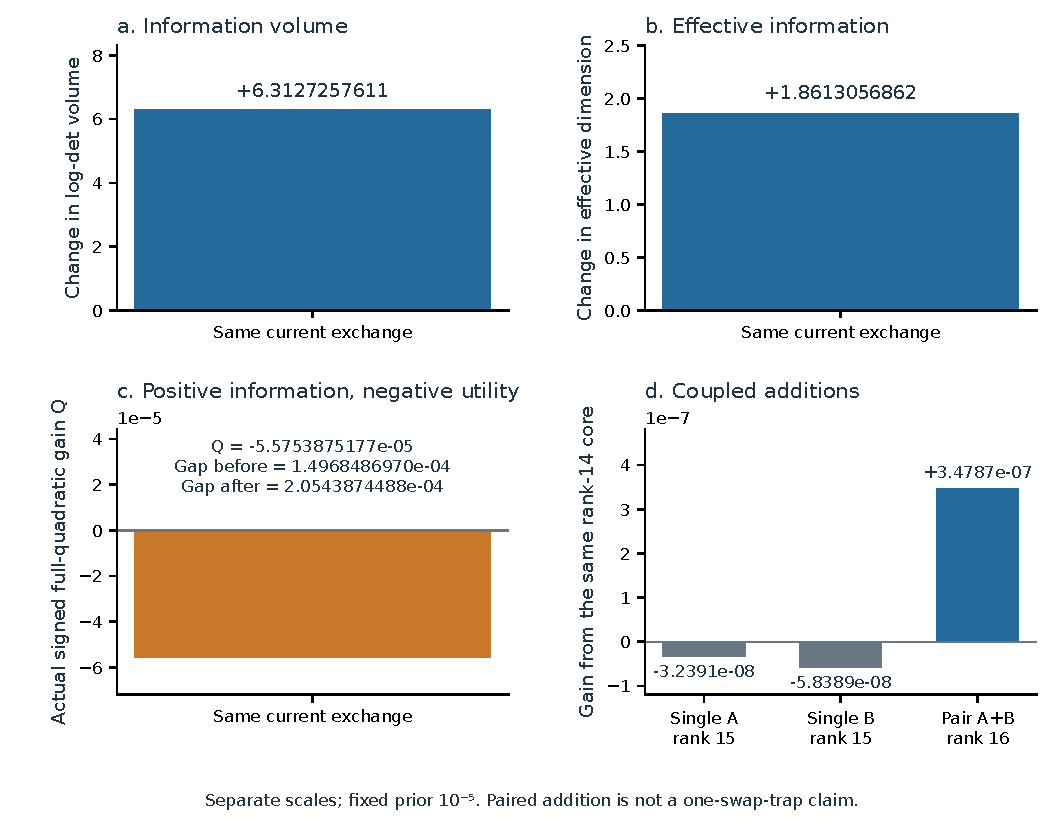
\includegraphics[width=.9\textwidth]{figures/information_and_pair_witness.pdf}
\caption{Two distinct witnesses. Increased information magnitude and slightly improved curvature fidelity coexist with negative material gain. Separately, two individually unfavorable additions become favorable when combined. The quantities have different units and are not combined into a universal score.}
\end{figure*}

\subsection{The cost of the actual finite displacement changes ordering}
A controlled $2\times2$ diagnostic separates the displacement from its evaluation. For common candidates, $v$ uses the old Hessian's first-order displacement and $d=s_n-s_o$ is the actual endpoint difference. Each is ranked by either its linear term or its full quadratic expression, and the selected replacement is evaluated using its actual $d$.

When a top-one action is mandatory and no-op is deliberately removed, the linear score $-g_F^Td$ selects a negative-gain replacement in 29 of 36 cells. Including $-\tfrac12d^TH_Fd$ reduces this count to 1 of 36. Finite-displacement curvature cost materially changes candidate ordering in these cases. The counts describe the controlled diagnostic; deployed conditional exchange separately rejects unfavorable checked actions. An older finite/first-order risk ratio also changed displacement construction and terminal search, and is not used to attribute an improvement to the curvature term alone.
